\chapter{Additions to the evaluation}\label{chpt:evaluationAdditions}
\glsresetall

\section{Training metrics}\label{sec:ea:trainingMetrics}

\begin{longtable}{p{0.03\textwidth}p{0.17\textwidth}p{0.03\textwidth}p{0.14\textwidth}p{0.03\textwidth}S[table-format=1.3]S[table-format=1.3]S[table-format=1.3]S[table-format=1.4]}
	\caption[Overview of all metric results.]{Overview of metric results for different training tasks and data splits.}\label{tab:ea:metricResults} \\
	\toprule
	&  \multicolumn{1}{c}{Training task} &&  \multicolumn{1}{c}{Epoch} && \multicolumn{1}{c}{$P$} & \multicolumn{1}{c}{$R$} & \multicolumn{1}{c}{$mAP_{50}$} & \multicolumn{1}{c}{$mAP_{50-95}$} \\
	\midrule
	\endfirsthead
	%
	\toprule
	&  \multicolumn{1}{c}{Training task} &&  \multicolumn{1}{c}{Epoch} && \multicolumn{1}{c}{$P$} & \multicolumn{1}{c}{$R$} & \multicolumn{1}{c}{$mAP_{50}$} & \multicolumn{1}{c}{$mAP_{50-95}$} \\
	\midrule
	\endhead
	%
	\multicolumn{9}{l}{\bfseries{Model 1, Validation data}} \\[7pt]
	%
	&  \multicolumn{1}{c}{\textsc{train}} &&  \multicolumn{1}{c}{\textsc{last}} && 0.975 & 0.982 & 0.988 & 0.675 \\[5pt]
	&  \multicolumn{1}{c}{\textsc{train}} &&  \multicolumn{1}{c}{\textsc{best}} && 0.982 & 0.974 & 0.988 & 0.664 \\[9pt]
	%
	&  \multicolumn{1}{c}{\textsc{finetune}} &&  \multicolumn{1}{c}{\textsc{last}} && 0.994 & 0.988 & 0.995 & 0.823 \\[5pt]
	&  \multicolumn{1}{c}{\textsc{finetune}} &&  \multicolumn{1}{c}{\textsc{best}} && 0.993 & 0.988 & 0.995 & 0.825 \\[7pt]
	%
	\multicolumn{9}{l}{\bfseries{Model 1, Test data}} \\[7pt]
	%
	&  \multicolumn{1}{c}{\textsc{train}} &&  \multicolumn{1}{c}{\textsc{last}} && 0.973 & 0.982 & 0.99  & 0.668 \\[5pt]
	&  \multicolumn{1}{c}{\textsc{train}} &&  \multicolumn{1}{c}{\textsc{best}} && 0.974 & 0.977 & 0.991 & 0.661 \\[9pt]
	%
	&  \multicolumn{1}{c}{\textsc{finetune}} &&  \multicolumn{1}{c}{\textsc{0}} && 0.254 & 0.977 & 0.254 & 0.0684 \\[5pt]
	&  \multicolumn{1}{c}{\textsc{finetune}} &&  \multicolumn{1}{c}{\textsc{5}} && 0.934 & 0.956 & 0.981 & 0.741  \\[5pt]
	&  \multicolumn{1}{c}{\textsc{finetune}} &&  \multicolumn{1}{c}{\textsc{10}} && 0.982 & 0.985 & 0.991 & 0.794  \\[5pt]
	&  \multicolumn{1}{c}{\textsc{finetune}} &&  \multicolumn{1}{c}{\textsc{15}} && 0.983 & 0.983 & 0.992 & 0.807  \\[5pt]
	&  \multicolumn{1}{c}{\textsc{finetune}} &&  \multicolumn{1}{c}{\textsc{20}} && 0.98  & 0.986 & 0.991 & 0.81   \\[5pt]
	&  \multicolumn{1}{c}{\textsc{finetune}} &&  \multicolumn{1}{c}{\textsc{25}} && 0.98  & 0.988 & 0.992 & 0.813  \\[5pt]
	&  \multicolumn{1}{c}{\textsc{finetune}} &&  \multicolumn{1}{c}{\textsc{30}} && 0.982 & 0.985 & 0.992 & 0.813  \\[5pt]
	&  \multicolumn{1}{c}{\textsc{finetune}} &&  \multicolumn{1}{c}{\textsc{35}} && 0.982 & 0.986 & 0.993 & 0.815  \\[5pt]
	&  \multicolumn{1}{c}{\textsc{finetune}} &&  \multicolumn{1}{c}{\textsc{40}} && 0.979 & 0.99  & 0.993 & 0.816  \\[5pt]
	&  \multicolumn{1}{c}{\textsc{finetune}} &&  \multicolumn{1}{c}{\textsc{45}} && 0.979 & 0.991 & 0.993 & 0.815  \\[5pt]
	&  \multicolumn{1}{c}{\textsc{finetune}} &&  \multicolumn{1}{c}{\textsc{50}} && 0.979 & 0.992 & 0.994 & 0.816  \\[5pt]
	&  \multicolumn{1}{c}{\textsc{finetune}} &&  \multicolumn{1}{c}{\textsc{55}} && 0.981 & 0.991 & 0.994 & 0.811  \\[5pt]
	&  \multicolumn{1}{c}{\textsc{finetune}} &&  \multicolumn{1}{c}{\textsc{60}} && 0.979 & 0.992 & 0.994 & 0.817  \\[5pt]
	&  \multicolumn{1}{c}{\textsc{finetune}} &&  \multicolumn{1}{c}{\textsc{65}} && 0.979 & 0.99  & 0.994 & 0.82   \\[5pt]
	&  \multicolumn{1}{c}{\textsc{finetune}} &&  \multicolumn{1}{c}{\textsc{70}} && 0.981 & 0.992 & 0.994 & 0.815  \\[5pt]
	&  \multicolumn{1}{c}{\textsc{finetune}} &&  \multicolumn{1}{c}{\textsc{75}} && 0.98  & 0.992 & 0.994 & 0.815  \\[5pt]
	&  \multicolumn{1}{c}{\textsc{finetune}} &&  \multicolumn{1}{c}{\textsc{80}} && 0.981 & 0.99  & 0.994 & 0.817  \\[5pt]
	&  \multicolumn{1}{c}{\textsc{finetune}} &&  \multicolumn{1}{c}{\textsc{85}} && 0.981 & 0.991 & 0.994 & 0.817  \\[5pt]
	&  \multicolumn{1}{c}{\textsc{finetune}} &&  \multicolumn{1}{c}{\textsc{90}} && 0.98  & 0.991 & 0.994 & 0.82   \\[5pt]
	&  \multicolumn{1}{c}{\textsc{finetune}} &&  \multicolumn{1}{c}{\textsc{95}} && 0.981 & 0.991 & 0.994 & 0.82   \\[5pt]
	%
	&  \multicolumn{1}{c}{\textsc{finetune}} &&  \multicolumn{1}{c}{\textsc{last}} && 0.98  & 0.992 & 0.994 & 0.819 \\[5pt]
	&  \multicolumn{1}{c}{\textsc{finetune}} &&  \multicolumn{1}{c}{\textsc{best}} && 0.981 & 0.991 & 0.994 & 0.819 \\[7pt]
	%
	\multicolumn{9}{l}{\bfseries{Model 2, Validation data}} \\[7pt]
	%
	&  \multicolumn{1}{c}{\textsc{train}} &&  \multicolumn{1}{c}{\textsc{last}} && 0.987 & 0.991 & 0.993 & 0.68 \\[5pt]
	&  \multicolumn{1}{c}{\textsc{train}} &&  \multicolumn{1}{c}{\textsc{best}} && 0.985 & 0.992 & 0.993 & 0.682 \\[7pt]
	%
	\multicolumn{9}{l}{\bfseries{Model 2, Test data}} \\[7pt]
	%
	&  \multicolumn{1}{c}{\textsc{train}} &&  \multicolumn{1}{c}{\textsc{last}} &&  0.984 & 0.986 & 0.991 & 0.673 \\[5pt]
	&  \multicolumn{1}{c}{\textsc{train}} &&  \multicolumn{1}{c}{\textsc{best}} &&  0.983 & 0.99  & 0.991 & 0.676 \\
	%
	\bottomrule
\end{longtable}

\newpage

\section{Inference results}\label{sec:ea:inferenceResults}

\begin{figure}[H]
	\centering
	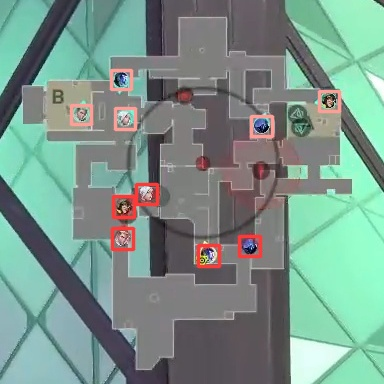
\includegraphics[width=0.8\linewidth]{images/a02-detect}
	\caption[Detected bounding boxes.]{Detected bounding boxes for a not trained image from the map "Ascent".}
	\label{fig:ea:outDetect}
\end{figure}

\begin{figure}[H]
	\centering
	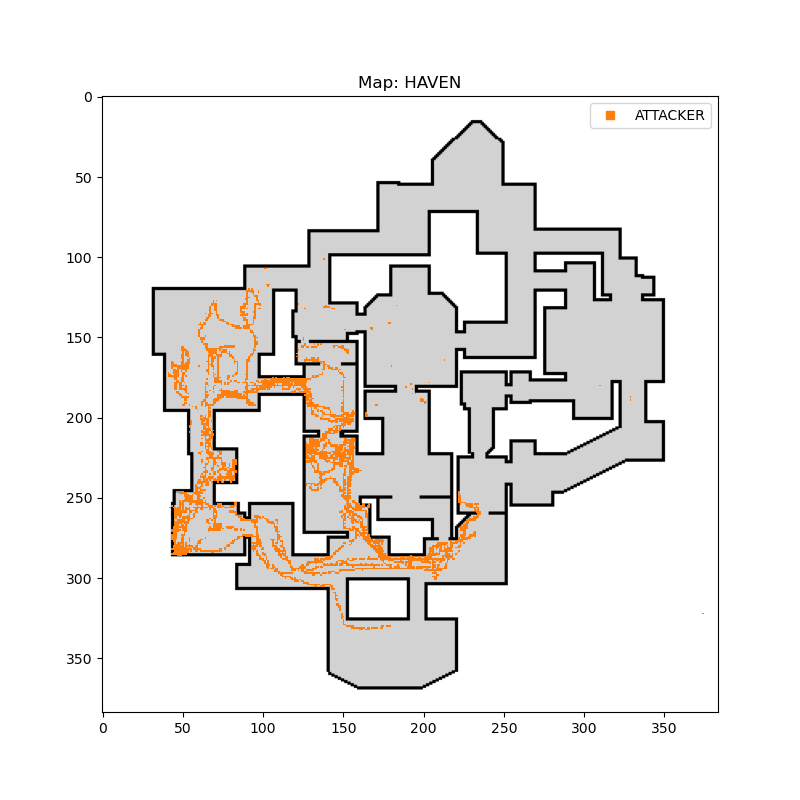
\includegraphics[width=0.95\linewidth]{images/a03-att-output}
	\caption[Output representation as map for attacker.]{Output representation as map, summarizing all positions 
		of attacker agents during one round on the map "Haven".}
	\label{fig:ea:outputAtt}
\end{figure}

\begin{figure}[H]
	\centering
	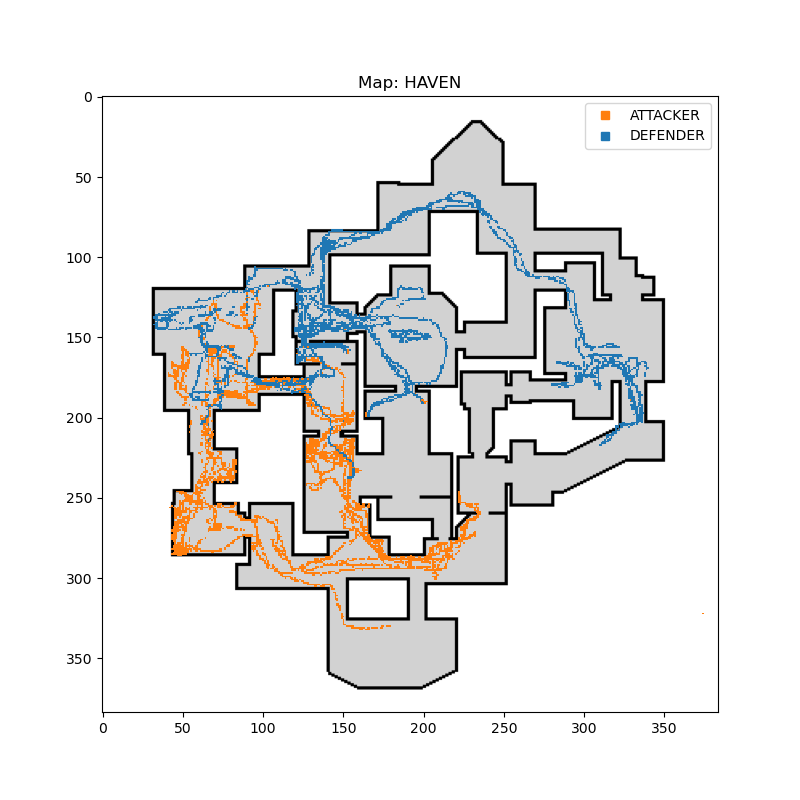
\includegraphics[width=0.95\linewidth]{images/a04-comb-output}
	\caption[Output representation as map.]{Output representation as map, summarizing all positions 
		of defender and attacker agents during one round on the map "Haven".}
	\label{fig:ea:outputComb}
\end{figure}